\section{Removing Look-up Structures}

Now that we can freely retrieve large array structures, we can focus on other
types of storage variables. A challenge we faced is that the protocol of
NIPoPoWs dependents on a Directed Acyclic Graph (DAG) of blocks which is a
mutable hashmap. This DAG is needed because interlink of superblocks can be
adversarially defined. Using it, simple graph search extract the set of
ancestor blocks of a block. In the final predicate evaluation, the set of
ancestors of the best blockchain tip is passed to the predicate. The
ancestors are included to avoid an adversary who presents an honest chain but
skips the blocks of interest.

This logic is intuitive and efficient to implement in most traditional
programming languages such as C++, JAVA, Python, JavaScript, etc. However, as
our analysis demonstrates, such an implementation in Solidity is significantly
expensive. Albeit Solidity supports hashmap look-up structures, hashmaps can
only be contained in storage. This affects performance, especially for large
proofs.

We make a keen observation regarding potential positions of the \emph{block of
interest} in the proof which lead us to the construction of an architecture
that does not require DAG, ancestors or other complementary structures. We
adopt the notation from~\cite{nipopows} to demonstrate our claims.
Additionally, we denote the initially submitted proof as $\pis$ and the
contesting proof as $\pic$. In this context, we consider the predicate $\pred$
to be of type "block $\boi$ exists inside a proof", where $\boi$ denotes
the block of interest. The entity that initiates a submission is $\es$, and the
entity that initiates a contest is $\ec$.

\noindent \textbf{Position of block of interest.} NIPoPoWs are sets of sampled
interlinked blocks, which means that they can be perceived as chains. If
$\pr_1$ differs from $\pr_2$, then a fork is created at the index of the last
common ancestor ($\lca$). The block of interest lies at a certain index within
$\pis$ and indicates a stable predicate~\cite{nipopows, generic-client} that is
true for $\pi_{subm}$. A submission in which $\boi$ is absent from $\pis$ is
aimless, because it automatically fails since no element of $\pis$ satisfies
$\pred$. On the contrary, $\pic$, tries to prove the falseness of the
underlying predicate. This means that, if the block of interest is included in
$\pi_{cont}$, then the contest is aimless. We refer to such aimless actions as
\emph{irrational} and components that are included in such actions as
irrational components, i.e.  irrational proof, blocks etc. We use the term
\emph{rational} to describe non-irrational actions and components.

\newcommand{\block}{\mathsf{B}}

In the NIPoPoW protocol, proofs' segments $\pis\{{{:}}\lca\}$ and $\pic\{{:}\lca\}$
are merged to prevent adversaries from skipping or adding blocks, and the
predicate is evaluated against $\pis\{{:}\lca\} \cup \pic\{{:}\lca\}$. We observe
that $\pic\{{:}\lca\}$ can be omitted, because no block $\block$ exists such that
\{$\block : \block \notin \pis\{{:}\lca\} \land \block \in \pic\{{:}\lca\}$\} where
$\block$ results into positive evaluation of the predicate. This is due to the
fact that, in a rational contest, $\boi$ is not included in $\pic$.
Consequently, $\pic$ is only rational if it forks $\pis$ in a block is prior
to $\boi$.

\renewcommand{\block}{}

\begin{figure}[h]
    \begin{center}
        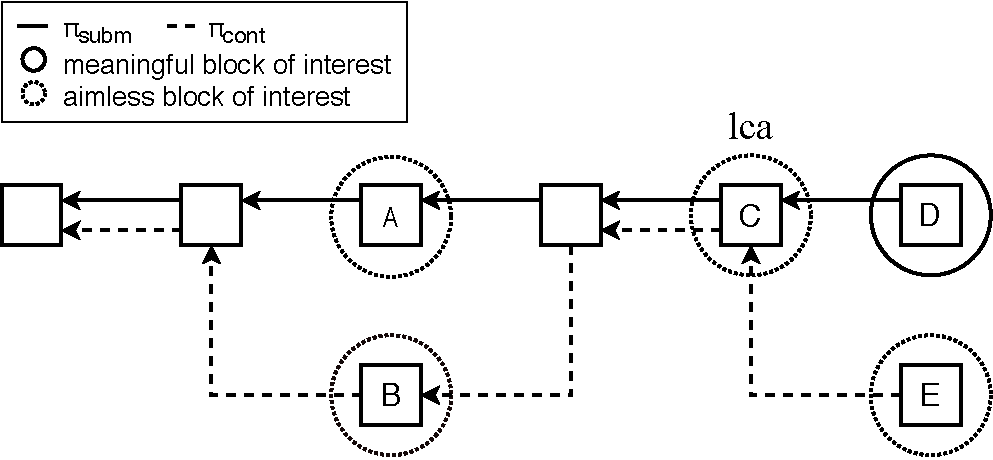
\includegraphics[width=1\columnwidth]{figures/boi-position.pdf}
    \end{center}
    \caption{Fork of two chains. Solid lines connect blocks of $\pis$
    and dashed lines connect blocks of $\pi_{cont}$. In this configuration,
    blocks in dashed circles are irrational blocks of interest, and the block
    in the solid circle is a rational block of interest. Blocks B, C and E are
    irrational because they exist in $\pic$. Block A is irrational because it
    belongs to the subchain $\pis\{{:}\lca\}$}
    \label{fig:boi-position}
\end{figure}

In Figure~\ref{fig:boi-position} we display a fork of two proofs. Solid lines
connect blocks of $\pis$ and dashed lines connect blocks of $\pic$.  Examining
which scenarios are rational depending on different positions of the block of
interest, we observe that blocks \texttt{B}, \texttt{C} and \texttt{E} do not
qualify, because they are included only in $\pic$. Block \texttt{A} is included
in $\pis\{{:}\lca\}$, which means that $\pic$ is an irrational contest because
the $\lca$ comes after $\boi$. Therefore A is an irrational block as a component
of an irrational contest. Given this configuration, the only rational block of
interest is \texttt{D} and its predecessors (which we do not display in the
figure).

\noindent \textbf{Minimal forks.} By combining the above observations, we
derive that, $\pic$ can be truncated into $\pic\{{:}\lca\}$ without
affecting the correctness of the protocol. We will term this truncated proof
$\pitr$\footnote{We cannot proceed to further truncation of $\pitr$, because
in the NIPoPoW protocol blocks within segment $\pi\{{:}\lca\}$ of each proof
are required for the score calculation.}. Security is preserved if we require
$\pitr$ to be a \emph{minimal fork} of $\pis$. A minimal fork is a fork chain
that shares exactly one common block with the main chain. A proof $\tilde\pi$,
which is minimal fork of $\pi$, has the following attributes:

\begin{enumerate}
\item $\pi\{lca\} = \tilde\pi[0]$
\item $\pi\{lca{:}\} \cap \tilde\pi[1{:}] = \O$
\end{enumerate}

By requiring $\pitr$ to be a minimal fork of $\pis$, we prevent adversaries
from dispatching an augmented $\pitr$ to claim better score against $\pis$.
Such an attempt is displayed in Figure~\ref{fig:adversary-minimal-fork}.

\begin{figure}[h]
    \begin{center}
        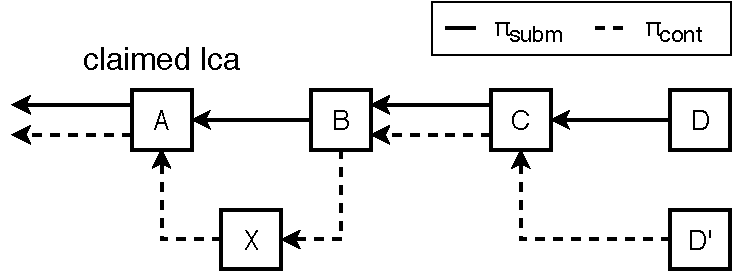
\includegraphics[width=0.7\columnwidth]{figures/adversary-minimal-fork.pdf}
    \end{center}

    \caption{An adversary attests to contest with a malformed proof. Adversary
        proof consists of blocks \{A, X, B, C, D'\} that achieves better score
        against submit proof \{A, B, C, D\}. This attempt is rejected due to
        the minimal-fork requirement.}

    \label{fig:adversary-minimal-fork}
\end{figure}

In Algorithm~\ref{alg:minimal-fork}, we show how minimal fork technique is
incorporated into our client replacing the DAG and ancestors. In
Figure~\ref{fig:minimal-fork} we show how the performance of the client
improves. We use the same test case as in \emph{hash-and-resubmit}.

\renewcommand{\genesis}{\textsf{G}}

\begin{algorithm}

    \label{alg:minimal-fork}
    \caption{The \textsf{NIPoPoW} client using the minimal fork technique}

    \begin{algorithmic}[1]

    \Contract{crosschain}
    \State $\textsf{events} \gets \bot;$ $\genesis \gets \bot$
    \Function{\sf initialize}{$\genesis_{remote}$}
        \State \genesis $\gets \genesis_{remote}$
    \EndFunction
    \Function{\sf submit}{$\pis$, $e$}
        \State \textsf{require}($\pis$[0] = $\genesis$)
        \State \textsf{require}($\textsf{events$[e]$} = \bot$)
        \State \textsf{require}($\textsf{valid-interlink}(\pis)$)
        \State \textsf{events$[e]$.hash} $\gets$ \textsf{H}($\pis$)
        \State \textsf{events$[e]$.pred} $\gets$
        \textsf{evaluate-predicate}(\textsf{$\pis$}, $e$)
    \EndFunction
    \Function{\sf contest}{$\pisa$, $\pitr$, $e$, $f$}
        \Comment{$f$: fork index}
        \State \textsf{require}($\pitr$[0] = $\pisa[f]$)
        \Comment{check fork head}
        \State \textsf{require}(\textsf{events}$[e]$ $\ne$ $\bot$)
        \State \textsf{require}(\textsf{events$[e]$.hash} $=$ \textsf{H}($\pisa$))
        \State \textsf{require}(\textsf{valid-interlink}($\pitr$))
        \State \textsf{require}(\textsf{minimal-fork}($\pisa$,
        $\pitr$, $f$))
        \State \textsf{require}(\textsf{score}($\pitr$)
            $>$ \textsf{score}($\pisa[f:]$))
        \State \textsf{events$[e]$.pred} $\gets$
            \textsf{evaluate-predicate}($\pitr$, $e$)
    \EndFunction
    \Function{\sf minimal-fork}{$\pi_1$, $\pi_2$, $f$}
        \For{$p\ in\ \pi_1$}
            \If{$p \in \pi_2$}
                \State\Return false
            \EndIf
        \EndFor
    \EndFunction
    \EndContract
    \vskip8pt
    \end{algorithmic}
\end{algorithm}



\begin{figure}[h]
    \begin{center}
        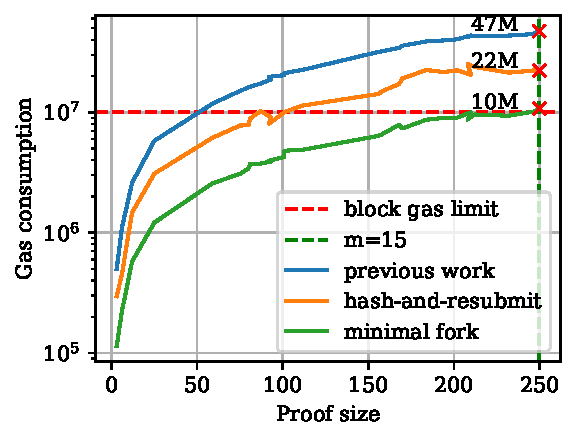
\includegraphics[width=1\columnwidth]{figures/minimal-fork.pdf}
    \end{center}
    \caption{}
    \label{fig:minimal-fork}
\end{figure}
